% =====================================================================
% Parte 08 — §2.8 Funciones uno a uno y sus inversas (Stewart, 7.ª ed.)
%
% Ejercicios elegidos (número del libro — página del libro):
%   9  (p. 226)  ¿Función uno a uno? — gráfica dada (recta horizontal)
%   13 (p. 226)  ¿Función uno a uno? — f(x) = -2x + 4
%   17 (p. 226)  ¿Función uno a uno? — h(x) = x^2 - 2x
%   25 (p. 226)  Valores de una función inversa
%   31 (p. 226)  Valores de una inversa a partir de una tabla
%   39 (p. 226)  Propiedad de la función inversa — f = 3x+4, g = (x-4)/3
%   43 (p. 226)  Propiedad de la función inversa — f = x^2-9 (x>=0), g = sqrt(x+9)
%   49 (p. 227)  Inversa de f(x) = 3x + 5
%   55 (p. 227)  Inversa de f(x) = x/(x+4)   (racional)
%   61 (p. 227)  Inversa de f(x) = 4 - x^2, x >= 0  (dominio restringido)
%   67 (p. 227)  Inversa de f(x) = sqrt(5+8x)
%   69 (p. 227)  Inversa de f(x) = 2 + raíz cúbica de x
%   73 (p. 227)  Trazar la gráfica de la inversa — f(x) = sqrt(x+1)
%   87 (p. 227)  Restringir el dominio — h(x) = (x+2)^2  (gráfica dada)
%   93 (p. 227)  Aplicación: costo de una pizza
%
% Figuras: fig_p08_09.png (ej. 9), fig_p08_87.png (ej. 87)
% =====================================================================

\documentclass[11pt]{article}
\usepackage[utf8]{inputenc}
\usepackage[spanish]{babel}
\usepackage[margin=2.3cm]{geometry}
\usepackage{amsmath,amssymb}
\usepackage{enumitem}
\usepackage{tcolorbox}
\tcbuselibrary{skins,breakable}
\usepackage{pgfplots}
\pgfplotsset{compat=1.18}
\usepackage{tikz}
\usepackage{graphicx}
\usepackage{array}
\usepackage[hidelinks]{hyperref}

% Notación española opcional (descomenta si quieres \sen en lugar de \sin)
% \DeclareMathOperator{\sen}{sen}
% \DeclareMathOperator{\tg}{tg}
% \DeclareMathOperator{\ctg}{ctg}

\newtcolorbox{sol}{colback=blue!5,colframe=blue!50!black,title=Solución paso a paso,breakable}
\newtcolorbox{teo}{colback=orange!8,colframe=orange!70!black,title=Teoría,breakable}
\newtcolorbox{nota}{colback=green!5,colframe=green!50!black,title=Idea clave,breakable}
\newtcolorbox{tip}{colback=yellow!10,colframe=yellow!60!black,title=Consejo,breakable}
\newtcolorbox{resp}{colback=red!5,colframe=red!50!black,title=Respuesta,breakable}
\newtcolorbox{reg}{colback=red!5,colframe=red!60!black,title=Regla,breakable}
\newtcolorbox{paso}[1]{colback=gray!5,colframe=gray!50!black,title={#1},breakable}

\graphicspath{{../images/}{images/}}
\newcommand{\sen}{\operatorname{sen}}

% babel spanish activa < y > y rompe TikZ/pgfplots (->, >=stealth)
\AtBeginDocument{\shorthandoff{<>}}

\begin{document}

\section*{Parte 08 --- Funciones uno a uno y sus inversas (Stewart §2.8, pp. 219--228)}

\begin{teo}
\textbf{Método de la sección.}
\begin{enumerate}[nosep,leftmargin=1.6em]
  \item \textbf{¿Es uno a uno?} Algebraicamente: suponer $f(x_1)=f(x_2)$ y deducir $x_1=x_2$. Si en cambio se exhiben $x_1\neq x_2$ con la misma imagen, no lo es.
  \item \textbf{Prueba de la recta horizontal.} $f$ es uno a uno si y sólo si ninguna recta horizontal corta su gráfica más de una vez.
  \item \textbf{Definición de inversa.} Si $f$ es uno a uno con dominio $A$ y rango $B$, entonces $f^{-1}(y)=x \iff f(x)=y$; además $\text{dom}(f^{-1})=\text{ran}(f)$ y $\text{ran}(f^{-1})=\text{dom}(f)$.
  \item \textbf{Cómo hallarla.} (i) Escriba $y=f(x)$. (ii) Despeje $x$ en términos de $y$. (iii) Intercambie $x$ y $y$; lo que queda es $y=f^{-1}(x)$.
  \item \textbf{Verificación.} $f^{-1}(f(x))=x$ para todo $x\in A$ y $f(f^{-1}(x))=x$ para todo $x\in B$. Cualquier función que cumpla ambas es la inversa.
  \item \textbf{Gráfica.} La gráfica de $f^{-1}$ es la reflexión de la de $f$ en la recta $y=x$, porque $(a,b)\in f \iff (b,a)\in f^{-1}$.
\end{enumerate}
\end{teo}

\begin{tip}
Se repiten en toda la parte:
\begin{itemize}[nosep,leftmargin=1.4em]
  \item $\sqrt{x^2}=|x|$, que vale $x$ sólo si $x\ge 0$: por eso las cuadráticas necesitan dominio restringido.
  \item Raíz par: el radicando debe ser $\ge 0$ y la raíz \emph{devuelve} un valor $\ge 0$. Raíz cúbica: sin restricción.
  \item $f^{-1}(x)$ \textbf{no} es $1/f(x)$; el $-1$ no es exponente.
  \item Una función creciente en todo su dominio (o decreciente en todo su dominio) es uno a uno.
  \item Racionales: para despejar $x$ de $y=\frac{ax+b}{cx+d}$, multiplique en cruz, agrupe los términos con $x$ y factorice $x$.
\end{itemize}
\end{tip}

% =====================================================================
\subsection*{Ejercicio 1 --- Prueba de la recta horizontal (libro 9, p. 226)}

\begin{quote}
\textbf{7--12} $\blacksquare$ \textbf{¿Función uno a uno?} Se da la gráfica de una función $f$. Determine si $f$ es uno a uno.

\textbf{9.}
\begin{center}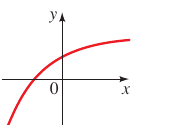
\includegraphics[width=0.34\textwidth]{fig_p08_09.png}\end{center}
\end{quote}

\begin{paso}{Paso 1 --- Aplico la prueba de la recta horizontal}
\textbf{Qué hago:} trazo mentalmente rectas horizontales $y=k$ sobre la gráfica dada y cuento cortes.

\textbf{¿De dónde sale?} De la gráfica del enunciado: una curva que sube de izquierda a derecha en todo el intervalo mostrado, sin tramos horizontales ni retrocesos.

\textbf{¿Por qué?} Prueba de la recta horizontal: $f$ es uno a uno si y sólo si ninguna recta horizontal corta la gráfica más de una vez.
\end{paso}

\begin{paso}{Paso 2 --- Conteo de cortes y conclusión}
\textbf{Qué hago:} verifico que cada $y=k$ corta la curva exactamente una vez.

\textbf{¿De dónde sale?} De la monotonía observada en el Paso 1: la curva es creciente, así que una vez que alcanza la altura $k$ nunca vuelve a ella.

\textbf{¿Por qué?} Toda función creciente en su dominio es uno a uno (resultado enunciado en la sección, tras el ejemplo 1).
\end{paso}

\begin{resp}
Sí, $f$ es uno a uno: es creciente y ninguna recta horizontal la corta más de una vez.
\end{resp}

% =====================================================================
\subsection*{Ejercicio 2 --- Uno a uno de una función lineal (libro 13, p. 226)}

\begin{quote}
\textbf{13--24} $\blacksquare$ \textbf{¿Función uno a uno?} Determine si la función es uno a uno.

\textbf{13.} $f(x)=-2x+4$
\end{quote}

\begin{paso}{Paso 1 --- Supongo imágenes iguales}
\textbf{Qué hago:} planteo $f(x_1)=f(x_2)$ y sustituyo la fórmula.

\textbf{¿De dónde sale?} Del enunciado: $f(x)=-2x+4$.

\textbf{¿Por qué?} Forma equivalente de la definición: si $f(x_1)=f(x_2)$ obliga a $x_1=x_2$, entonces $f$ es uno a uno.
\[
-2x_1+4=-2x_2+4.
\]
\end{paso}

\begin{paso}{Paso 2 --- Despejo}
\textbf{Qué hago:} resto $4$ y divido entre $-2$ en ambos lados.

\textbf{¿De dónde sale?} De la ecuación del Paso 1.

\textbf{¿Por qué?} Son operaciones inversas válidas en toda ecuación; dividir entre $-2\neq 0$ está permitido.
\[
-2x_1=-2x_2 \;\Longrightarrow\; x_1=x_2.
\]
\end{paso}

\begin{resp}
$f(x)=-2x+4$ \textbf{es uno a uno} (toda lineal con pendiente $m\neq 0$ lo es).
\end{resp}

% =====================================================================
\subsection*{Ejercicio 3 --- Una cuadrática no es uno a uno (libro 17, p. 226)}

\begin{quote}
\textbf{17.} $h(x)=x^2-2x$
\end{quote}

\begin{paso}{Paso 1 --- Busco dos entradas con la misma imagen}
\textbf{Qué hago:} factorizo $h(x)=x(x-2)$ para leer sus ceros.

\textbf{¿De dónde sale?} Del enunciado: $x^2-2x$ tiene factor común $x$.

\textbf{¿Por qué?} Los ceros son entradas distintas con la misma imagen $0$, que es justo el contraejemplo que buscamos.
\[
h(x)=x(x-2)=0 \iff x=0 \ \text{ó}\ x=2.
\]
\end{paso}

\begin{paso}{Paso 2 --- Contraejemplo explícito}
\textbf{Qué hago:} evalúo en $x=0$ y $x=2$.

\textbf{¿De dónde sale?} De los ceros del Paso 1.

\textbf{¿Por qué?} La definición se niega exhibiendo $x_1\neq x_2$ con $h(x_1)=h(x_2)$; no hace falta más.
\[
h(0)=0^2-2(0)=0, \qquad h(2)=2^2-2(2)=4-4=0.
\]
\end{paso}

\begin{resp}
$h$ \textbf{no es uno a uno}: $h(0)=h(2)=0$ con $0\neq 2$. (Su gráfica es una parábola y la recta $y=0$ la corta dos veces.)
\end{resp}

% =====================================================================
\subsection*{Ejercicio 4 --- Leer valores de $f^{-1}$ desde la definición (libro 25, p. 226)}

\begin{quote}
\textbf{25--28} $\blacksquare$ \textbf{Encontrar valores de una función inversa} Suponga que $f$ es una función uno a uno.

\textbf{25.} \textit{a}) Si $f(2)=7$, encuentre $f^{-1}(7)$.

\hspace{1.2em}\textit{b}) Si $f^{-1}(3)=-1$, encuentre $f(-1)$.
\end{quote}

\begin{paso}{Paso 1 --- Inciso a)}
\textbf{Qué hago:} aplico la definición $f^{-1}(y)=x \iff f(x)=y$ con $x=2$, $y=7$.

\textbf{¿De dónde sale?} Del dato $f(2)=7$.

\textbf{¿Por qué?} Definición de la inversa: $f^{-1}$ devuelve la entrada que produjo esa salida.
\[
f(2)=7 \iff f^{-1}(7)=2.
\]
\end{paso}

\begin{paso}{Paso 2 --- Inciso b)}
\textbf{Qué hago:} uso la misma equivalencia leída de derecha a izquierda, con $x=-1$, $y=3$.

\textbf{¿De dónde sale?} Del dato $f^{-1}(3)=-1$.

\textbf{¿Por qué?} La equivalencia de la definición es una doble implicación, así que se lee en ambos sentidos.
\[
f^{-1}(3)=-1 \iff f(-1)=3.
\]
\end{paso}

\begin{resp}
\textit{a}) $f^{-1}(7)=2$. \qquad \textit{b}) $f(-1)=3$.
\end{resp}

% =====================================================================
\subsection*{Ejercicio 5 --- Valores de la inversa desde una tabla (libro 31, p. 226)}

\begin{quote}
\textbf{31--36} $\blacksquare$ \textbf{Determinar valores de una inversa utilizando una tabla} Se da una tabla de valores para una función uno a uno. Encuentre los valores indicados.

\textbf{31.} $f^{-1}(5)$

\begin{center}
\begin{tabular}{|c|c|c|c|c|c|c|}
\hline
$x$ & 1 & 2 & 3 & 4 & 5 & 6 \\ \hline
$f(x)$ & 4 & 6 & 2 & 5 & 0 & 1 \\ \hline
\end{tabular}
\end{center}
\end{quote}

\begin{paso}{Paso 1 --- Busco la salida $5$ en la fila de $f(x)$}
\textbf{Qué hago:} recorro la fila $f(x)$ hasta hallar el valor $5$ y leo la $x$ que está arriba.

\textbf{¿De dónde sale?} De la tabla: $5$ aparece en la columna encabezada por $x=4$.

\textbf{¿Por qué?} Definición de inversa: $f^{-1}(5)$ es la única entrada cuya imagen es $5$, y la unicidad la garantiza que $f$ sea uno a uno.
\[
f(4)=5 \iff f^{-1}(5)=4.
\]
\end{paso}

\begin{resp}
$f^{-1}(5)=4$.
\end{resp}

% =====================================================================
\subsection*{Ejercicio 6 --- Verificar inversas: caso lineal (libro 39, p. 226)}

\begin{quote}
\textbf{37--48} $\blacksquare$ \textbf{Propiedad de función inversa} Utilice la propiedad de la función inversa para demostrar que $f$ y $g$ son inversas entre sí.

\textbf{39.} $f(x)=3x+4$; \quad $g(x)=\dfrac{x-4}{3}$
\end{quote}

\begin{paso}{Paso 1 --- Compongo $f\circ g$}
\textbf{Qué hago:} sustituyo $g(x)$ en el lugar de la variable de $f$.

\textbf{¿De dónde sale?} De las dos fórmulas del enunciado.

\textbf{¿Por qué?} La propiedad de la función inversa pide comprobar $f(g(x))=x$ para todo $x$ del dominio de $g$, que aquí es $\mathbb{R}$.
\[
f(g(x))=3\!\left(\frac{x-4}{3}\right)+4=(x-4)+4=x.
\]
\end{paso}

\begin{paso}{Paso 2 --- Compongo $g\circ f$}
\textbf{Qué hago:} sustituyo $f(x)$ en el lugar de la variable de $g$.

\textbf{¿De dónde sale?} De las mismas fórmulas.

\textbf{¿Por qué?} La propiedad exige \emph{las dos} cancelaciones; con una sola no basta para concluir que son inversas.
\[
g(f(x))=\frac{(3x+4)-4}{3}=\frac{3x}{3}=x.
\]
\end{paso}

\begin{resp}
$f(g(x))=x$ y $g(f(x))=x$ para todo $x\in\mathbb{R}$, luego $f$ y $g$ \textbf{son inversas entre sí}.
\end{resp}

% =====================================================================
\subsection*{Ejercicio 7 --- Verificar inversas con dominio restringido (libro 43, p. 226)}

\begin{quote}
\textbf{43.} $f(x)=x^2-9$, \ $x\ge 0$; \quad $g(x)=\sqrt{x+9}$, \ $x\ge -9$
\end{quote}

\begin{paso}{Paso 1 --- Compongo $f\circ g$}
\textbf{Qué hago:} sustituyo $g(x)=\sqrt{x+9}$ en $f$ y uso $(\sqrt{a})^2=a$ para $a\ge 0$.

\textbf{¿De dónde sale?} Del enunciado; el radicando $x+9$ es $\ge 0$ precisamente porque $x\ge -9$.

\textbf{¿Por qué?} La igualdad $(\sqrt{a})^2=a$ vale para todo $a\ge 0$, que es lo que garantiza la restricción dada.
\[
f(g(x))=\left(\sqrt{x+9}\right)^2-9=(x+9)-9=x, \qquad x\ge -9.
\]
\end{paso}

\begin{paso}{Paso 2 --- Compongo $g\circ f$ cuidando el valor absoluto}
\textbf{Qué hago:} sustituyo $f(x)=x^2-9$ en $g$ y aplico $\sqrt{x^2}=|x|$.

\textbf{¿De dónde sale?} De las fórmulas del enunciado; el $-9$ y el $+9$ se cancelan dentro de la raíz.

\textbf{¿Por qué?} $\sqrt{x^2}=|x|$ siempre, y $|x|=x$ únicamente cuando $x\ge 0$, que es la restricción impuesta a $f$.
\[
g(f(x))=\sqrt{(x^2-9)+9}=\sqrt{x^2}=|x|=x, \qquad x\ge 0.
\]
\end{paso}

\begin{resp}
Ambas cancelaciones se cumplen en los dominios indicados, así que $f$ y $g$ \textbf{son inversas entre sí}. Sin la restricción $x\ge 0$ fallaría: $g(f(-1))=\sqrt{1}=1\neq -1$.
\end{resp}

% =====================================================================
\subsection*{Ejercicio 8 --- Inversa de una función lineal (libro 49, p. 227)}

\begin{quote}
\textbf{49--70} $\blacksquare$ \textbf{Encontrar la función inversa} Encuentre la función inversa de $f$.

\textbf{49.} $f(x)=3x+5$
\end{quote}

\begin{paso}{Paso 1 --- Escribo $y=f(x)$ y despejo $x$}
\textbf{Qué hago:} aplico los pasos 1 y 2 del recuadro ``Cómo determinar la inversa'': resto $5$ y divido entre $3$.

\textbf{¿De dónde sale?} Del enunciado: $y=3x+5$.

\textbf{¿Por qué?} De la definición, $y=f(x) \iff f^{-1}(y)=x$; por eso despejar $x$ en términos de $y$ es exactamente hallar $f^{-1}$.
\[
y=3x+5 \;\Longrightarrow\; 3x=y-5 \;\Longrightarrow\; x=\frac{y-5}{3}.
\]
\end{paso}

\begin{paso}{Paso 2 --- Intercambio $x$ y $y$}
\textbf{Qué hago:} escribo la relación con la variable independiente llamada $x$.

\textbf{¿De dónde sale?} Del despeje del Paso 1.

\textbf{¿Por qué?} Paso 3 del método: el intercambio sólo renombra variables para dejar la inversa en la notación usual $y=f^{-1}(x)$.
\[
f^{-1}(x)=\frac{x-5}{3}.
\]
\end{paso}

\begin{paso}{Paso 3 --- Verificación en ambos sentidos}
\textbf{Qué hago:} compongo las dos maneras.

\textbf{¿De dónde sale?} De $f(x)=3x+5$ y del resultado del Paso 2.

\textbf{¿Por qué?} Propiedad de la función inversa: si ambas composiciones dan $x$, el candidato es la inversa.
\[
f\!\left(f^{-1}(x)\right)=3\!\left(\frac{x-5}{3}\right)+5=x, \qquad
f^{-1}\!\left(f(x)\right)=\frac{(3x+5)-5}{3}=x.
\]
\end{paso}

\begin{resp}
$f^{-1}(x)=\dfrac{x-5}{3}$, con dominio y rango $\mathbb{R}$.
\end{resp}

% =====================================================================
\subsection*{Ejercicio 9 --- Inversa de una función racional (libro 55, p. 227)}

\begin{quote}
\textbf{55.} $f(x)=\dfrac{x}{x+4}$
\end{quote}

\begin{paso}{Paso 1 --- Quito el denominador}
\textbf{Qué hago:} escribo $y=\dfrac{x}{x+4}$ y multiplico ambos lados por $x+4$.

\textbf{¿De dónde sale?} Del enunciado; el dominio de $f$ excluye $x=-4$, así que $x+4\neq 0$.

\textbf{¿Por qué?} Multiplicar por una cantidad distinta de cero preserva la ecuación, y es el primer movimiento del ejemplo 9 de la sección.
\[
y(x+4)=x \;\Longrightarrow\; yx+4y=x.
\]
\end{paso}

\begin{paso}{Paso 2 --- Agrupo los términos con $x$ y factorizo}
\textbf{Qué hago:} paso $yx$ a la derecha y saco $x$ como factor común.

\textbf{¿De dónde sale?} De la ecuación desarrollada del Paso 1.

\textbf{¿Por qué?} $x$ aparece en dos términos; factorizarlo es la única forma de despejarlo (ejemplo 9).
\[
4y=x-yx=x(1-y) \;\Longrightarrow\; x=\frac{4y}{1-y}, \quad y\neq 1.
\]
\end{paso}

\begin{paso}{Paso 3 --- Intercambio y verifico}
\textbf{Qué hago:} renombro variables y compongo $f\circ f^{-1}$.

\textbf{¿De dónde sale?} Del despeje del Paso 2.

\textbf{¿Por qué?} La propiedad de la función inversa confirma el resultado; la restricción $x\neq 1$ viene de que $y=1$ nunca es imagen de $f$.
\[
f^{-1}(x)=\frac{4x}{1-x};\qquad
f\!\left(\frac{4x}{1-x}\right)=\frac{\frac{4x}{1-x}}{\frac{4x}{1-x}+4}
=\frac{4x}{4x+4(1-x)}=\frac{4x}{4}=x.
\]
\end{paso}

\begin{resp}
$f^{-1}(x)=\dfrac{4x}{1-x}$, con dominio $\{x: x\neq 1\}$ (que es el rango de $f$) y rango $\{y: y\neq -4\}$.
\end{resp}

% =====================================================================
\subsection*{Ejercicio 10 --- Inversa de una cuadrática con dominio restringido (libro 61, p. 227)}

\begin{quote}
\textbf{61.} $f(x)=4-x^2$, \quad $x\ge 0$
\end{quote}

\begin{paso}{Paso 1 --- Despejo $x^2$}
\textbf{Qué hago:} escribo $y=4-x^2$ y aíslo $x^2$.

\textbf{¿De dónde sale?} Del enunciado.

\textbf{¿Por qué?} Es el paso 2 del método; todavía no se puede tomar raíz sin decidir el signo.
\[
y=4-x^2 \;\Longrightarrow\; x^2=4-y.
\]
\end{paso}

\begin{paso}{Paso 2 --- Tomo la raíz con el signo que impone el dominio}
\textbf{Qué hago:} aplico $\sqrt{x^2}=|x|$ y uso $x\ge 0$ para quedarme con la raíz positiva.

\textbf{¿De dónde sale?} De la restricción $x\ge 0$ del enunciado.

\textbf{¿Por qué?} Sin restringir, $4-x^2$ no es uno a uno ($f(1)=f(-1)=3$); la restricción es justo lo que hace único el despeje.
\[
|x|=\sqrt{4-y} \;\Longrightarrow\; x=\sqrt{4-y}, \qquad y\le 4.
\]
\end{paso}

\begin{paso}{Paso 3 --- Intercambio, dominio y verificación}
\textbf{Qué hago:} renombro variables y compongo en ambos sentidos.

\textbf{¿De dónde sale?} Del Paso 2; el rango de $f$ es $(-\infty,4]$ porque $x\ge 0$ da $x^2\ge 0$, luego $4-x^2\le 4$.

\textbf{¿Por qué?} $\text{dom}(f^{-1})=\text{ran}(f)$ y $\text{ran}(f^{-1})=\text{dom}(f)$, por la definición de inversa.
\[
f^{-1}(x)=\sqrt{4-x};\qquad
f\!\left(\sqrt{4-x}\right)=4-(4-x)=x,\qquad
f^{-1}\!\left(4-x^2\right)=\sqrt{x^2}=|x|=x \ \ (x\ge 0).
\]
\end{paso}

\begin{resp}
$f^{-1}(x)=\sqrt{4-x}$, con dominio $(-\infty,4]$ y rango $[0,\infty)$.
\end{resp}

% =====================================================================
\subsection*{Ejercicio 11 --- Inversa de una función con raíz cuadrada (libro 67, p. 227)}

\begin{quote}
\textbf{67.} $f(x)=\sqrt{5+8x}$
\end{quote}

\begin{paso}{Paso 1 --- Dominio y rango de $f$}
\textbf{Qué hago:} exijo $5+8x\ge 0$ y observo que la raíz cuadrada devuelve valores $\ge 0$.

\textbf{¿De dónde sale?} Del enunciado: el radicando es $5+8x$.

\textbf{¿Por qué?} La raíz de índice par sólo está definida para argumentos no negativos y su salida es no negativa; esto fija los dominios que usaremos después.
\[
5+8x\ge 0 \iff x\ge -\tfrac{5}{8}; \qquad \text{ran}(f)=[0,\infty).
\]
\end{paso}

\begin{paso}{Paso 2 --- Elevo al cuadrado y despejo $x$}
\textbf{Qué hago:} escribo $y=\sqrt{5+8x}$, elevo al cuadrado y despejo.

\textbf{¿De dónde sale?} De la fórmula del enunciado.

\textbf{¿Por qué?} Elevar al cuadrado es válido y reversible aquí porque ambos lados son $\ge 0$ (Paso 1).
\[
y^2=5+8x \;\Longrightarrow\; 8x=y^2-5 \;\Longrightarrow\; x=\frac{y^2-5}{8}, \quad y\ge 0.
\]
\end{paso}

\begin{paso}{Paso 3 --- Intercambio y verificación}
\textbf{Qué hago:} renombro y compongo.

\textbf{¿De dónde sale?} Del despeje del Paso 2 y de $\text{dom}(f^{-1})=\text{ran}(f)=[0,\infty)$.

\textbf{¿Por qué?} Propiedad de la función inversa.
\[
f^{-1}(x)=\frac{x^2-5}{8}, \ x\ge 0; \qquad
f\!\left(\frac{x^2-5}{8}\right)=\sqrt{5+(x^2-5)}=\sqrt{x^2}=x \ (x\ge0),
\]
\[
f^{-1}\!\left(\sqrt{5+8x}\right)=\frac{(5+8x)-5}{8}=x.
\]
\end{paso}

\begin{resp}
$f^{-1}(x)=\dfrac{x^2-5}{8}$, \ $x\ge 0$; su dominio es $[0,\infty)$ y su rango $\left[-\tfrac{5}{8},\infty\right)$.
\end{resp}

% =====================================================================
\subsection*{Ejercicio 12 --- Inversa con raíz cúbica (libro 69, p. 227)}

\begin{quote}
\textbf{69.} $f(x)=2+\sqrt[3]{x}$
\end{quote}

\begin{paso}{Paso 1 --- Aíslo la raíz cúbica}
\textbf{Qué hago:} escribo $y=2+\sqrt[3]{x}$ y resto $2$.

\textbf{¿De dónde sale?} Del enunciado.

\textbf{¿Por qué?} Para deshacer una raíz hay que dejarla sola antes de elevar a la potencia correspondiente.
\[
y-2=\sqrt[3]{x}.
\]
\end{paso}

\begin{paso}{Paso 2 --- Elevo al cubo}
\textbf{Qué hago:} elevo ambos lados a la tercera potencia.

\textbf{¿De dónde sale?} De la ecuación del Paso 1.

\textbf{¿Por qué?} La raíz cúbica está definida para todo real y $(\sqrt[3]{a})^3=a$ sin restricciones de signo, a diferencia de la raíz par.
\[
(y-2)^3=x.
\]
\end{paso}

\begin{paso}{Paso 3 --- Intercambio y verificación}
\textbf{Qué hago:} renombro variables y compongo en ambos sentidos.

\textbf{¿De dónde sale?} Del Paso 2.

\textbf{¿Por qué?} Propiedad de la función inversa; el dominio y el rango son $\mathbb{R}$ en ambas.
\[
f^{-1}(x)=(x-2)^3;\qquad
f\!\left((x-2)^3\right)=2+\sqrt[3]{(x-2)^3}=2+(x-2)=x,
\]
\[
f^{-1}\!\left(2+\sqrt[3]{x}\right)=\left(2+\sqrt[3]{x}-2\right)^3=\left(\sqrt[3]{x}\right)^3=x.
\]
\end{paso}

\begin{resp}
$f^{-1}(x)=(x-2)^3$, con dominio y rango $\mathbb{R}$.
\end{resp}

% =====================================================================
\subsection*{Ejercicio 13 --- Gráfica de la inversa como reflexión en $y=x$ (libro 73, p. 227)}

\begin{quote}
\textbf{71--74} $\blacksquare$ \textbf{Trazar la gráfica de una función inversa} Se da una función $f$. \textit{a}) Trace la gráfica de $f$. \textit{b}) Use la gráfica de $f$ para trazar la gráfica de $f^{-1}$. \textit{c}) Encuentre $f^{-1}$.

\textbf{73.} $f(x)=\sqrt{x+1}$
\end{quote}

\begin{paso}{Paso 1 --- Inciso a): gráfica de $f$ por transformación}
\textbf{Qué hago:} parto de $y=\sqrt{x}$ y la traslado $1$ unidad a la izquierda.

\textbf{¿De dónde sale?} Del enunciado: $\sqrt{x+1}$ es $\sqrt{x}$ con $x$ reemplazada por $x+1$.

\textbf{¿Por qué?} Transformaciones de la §2.6: $y=f(x+c)$ con $c>0$ traslada la gráfica $c$ unidades a la izquierda. Dominio $[-1,\infty)$, rango $[0,\infty)$.
\begin{center}
\begin{tabular}{|c|c|c|c|c|}
\hline
$x$ & $-1$ & $0$ & $3$ & $8$ \\ \hline
$f(x)$ & $0$ & $1$ & $2$ & $3$ \\ \hline
\end{tabular}
\end{center}
\end{paso}

\begin{paso}{Paso 2 --- Inciso b): reflejo en la recta $y=x$}
\textbf{Qué hago:} intercambio las coordenadas de los puntos de la tabla para obtener puntos de $f^{-1}$.

\textbf{¿De dónde sale?} De la tabla del Paso 1: $(-1,0)\mapsto(0,-1)$, $(0,1)\mapsto(1,0)$, $(3,2)\mapsto(2,3)$, $(8,3)\mapsto(3,8)$.

\textbf{¿Por qué?} $(a,b)$ está en la gráfica de $f$ si y sólo si $(b,a)$ está en la de $f^{-1}$, y ese intercambio es exactamente la reflexión en $y=x$.
\begin{center}
\begin{tikzpicture}
\begin{axis}[width=9.5cm,height=8cm,axis lines=middle,xlabel=$x$,ylabel=$y$,
  xmin=-2.5,xmax=6.5,ymin=-2.5,ymax=6.5,grid=both,grid style={gray!20},
  legend pos=north west,legend style={font=\footnotesize}]
\addplot[domain=-1:6,samples=100,thick,blue]{sqrt(x+1)};
\addlegendentry{$f(x)=\sqrt{x+1}$}
\addplot[domain=0:2.7,samples=100,thick,red]{x^2-1};
\addlegendentry{$f^{-1}(x)=x^2-1,\ x\ge 0$}
\addplot[domain=-2.2:6,samples=2,dashed,orange]{x};
\addlegendentry{$y=x$}
\end{axis}
\end{tikzpicture}
\end{center}
\end{paso}

\begin{paso}{Paso 3 --- Inciso c): ecuación de $f^{-1}$}
\textbf{Qué hago:} escribo $y=\sqrt{x+1}$ con $y\ge 0$, elevo al cuadrado y despejo $x$.

\textbf{¿De dónde sale?} Del enunciado; $y\ge 0$ porque la raíz cuadrada nunca es negativa.

\textbf{¿Por qué?} Método de los tres pasos, y la condición $y\ge 0$ se convierte tras el intercambio en la restricción $x\ge 0$ del dominio de $f^{-1}$.
\[
y^2=x+1 \;\Longrightarrow\; x=y^2-1 \;\xrightarrow{\ \text{intercambio}\ }\; f^{-1}(x)=x^2-1,\quad x\ge 0.
\]
\end{paso}

\begin{paso}{Paso 4 --- Verificación}
\textbf{Qué hago:} compongo en ambos sentidos.

\textbf{¿De dónde sale?} De $f(x)=\sqrt{x+1}$ y $f^{-1}(x)=x^2-1$ con $x\ge 0$.

\textbf{¿Por qué?} Propiedad de la función inversa.
\[
f\!\left(x^2-1\right)=\sqrt{x^2-1+1}=|x|=x \ (x\ge 0), \qquad
f^{-1}\!\left(\sqrt{x+1}\right)=\left(\sqrt{x+1}\right)^2-1=x \ (x\ge -1).
\]
\end{paso}

\begin{resp}
$f^{-1}(x)=x^2-1$, \ $x\ge 0$: la mitad derecha de la parábola $y=x^2-1$. Dominio $[0,\infty)$, rango $[-1,\infty)$.
\end{resp}

% =====================================================================
\subsection*{Ejercicio 14 --- Restringir el dominio para que exista inversa (libro 87, p. 227)}

\begin{quote}
\textbf{85--88} $\blacksquare$ \textbf{Restringir el dominio} La función dada no es uno a uno. Restrinja su dominio para que la función resultante \textit{sea} uno a uno. Encuentre la inversa de la función con el dominio restringido. (Hay más de una respuesta correcta.)

\textbf{87.} $h(x)=(x+2)^2$
\begin{center}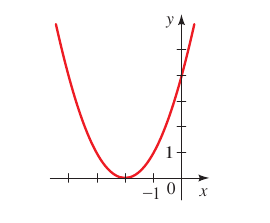
\includegraphics[width=0.42\textwidth]{fig_p08_87.png}\end{center}
\end{quote}

\begin{paso}{Paso 1 --- Localizo el vértice y elijo una mitad}
\textbf{Qué hago:} leo de la gráfica que la parábola tiene vértice en $(-2,0)$ y restrinjo a $x\ge -2$.

\textbf{¿De dónde sale?} De la forma $(x+2)^2$: es $y=x^2$ trasladada $2$ unidades a la izquierda (§2.6), lo que coincide con la gráfica dada.

\textbf{¿Por qué?} A cada lado del vértice la parábola es monótona, y una función monótona en su dominio es uno a uno; sobre todo $\mathbb{R}$ falla, pues $h(-1)=h(-3)=1$.
\end{paso}

\begin{paso}{Paso 2 --- Despejo con el signo correcto}
\textbf{Qué hago:} escribo $y=(x+2)^2$, tomo raíz usando $\sqrt{(x+2)^2}=|x+2|$ y aplico $x\ge -2$.

\textbf{¿De dónde sale?} De la restricción del Paso 1: $x\ge -2 \iff x+2\ge 0 \iff |x+2|=x+2$.

\textbf{¿Por qué?} Es lo que vuelve único el despeje; sin ello quedarían dos ramas y la inversa no estaría bien definida.
\[
|x+2|=\sqrt{y} \;\Longrightarrow\; x+2=\sqrt{y} \;\Longrightarrow\; x=\sqrt{y}-2, \qquad y\ge 0.
\]
\end{paso}

\begin{paso}{Paso 3 --- Intercambio y verificación}
\textbf{Qué hago:} renombro variables y compongo en ambos sentidos.

\textbf{¿De dónde sale?} Del Paso 2; el rango de $h$ restringida es $[0,\infty)$, así que ése es el dominio de $h^{-1}$.

\textbf{¿Por qué?} Propiedad de la función inversa, más $\text{dom}(h^{-1})=\text{ran}(h)$.
\[
h^{-1}(x)=\sqrt{x}-2;\qquad
h\!\left(\sqrt{x}-2\right)=\left(\sqrt{x}-2+2\right)^2=\left(\sqrt{x}\right)^2=x \ \ (x\ge0),
\]
\[
h^{-1}\!\left((x+2)^2\right)=\sqrt{(x+2)^2}-2=|x+2|-2=x \ \ (x\ge-2).
\]
\end{paso}

\begin{resp}
Con el dominio restringido $x\ge -2$: \ $h^{-1}(x)=\sqrt{x}-2$, dominio $[0,\infty)$ y rango $[-2,\infty)$.

\medskip
La otra respuesta válida es restringir a $x\le -2$, y entonces $h^{-1}(x)=-\sqrt{x}-2$.
\end{resp}

% =====================================================================
\subsection*{Ejercicio 15 --- Aplicación: costo de una pizza (libro 93, p. 227)}

\begin{quote}
\textbf{93. Costo de una pizza} Marcello's Pizza cobra un precio base de 16 dólares por una pizza grande más \$1.50 por cada ingrediente adicional.

\textit{a}) Encuentre una función $f$ que modele el precio de una pizza con $n$ ingredientes.

\textit{b}) Encuentre la inversa de la función $f$. ¿Qué representa $f^{-1}$?

\textit{c}) ¿Cuántos ingredientes tiene una pizza de 25 dólares?
\end{quote}

\begin{paso}{Paso 1 --- Inciso a): modelo lineal}
\textbf{Qué hago:} armo precio $=$ base $+$ (costo por ingrediente)$\cdot$(número de ingredientes).

\textbf{¿De dónde sale?} Del enunciado: base $16$ dólares y \$$1.50$ por cada ingrediente adicional.

\textbf{¿Por qué?} Un costo fijo más un costo constante por unidad es una función lineal (§2.5), con ordenada al origen $16$ y pendiente $1.5$.
\[
f(n)=16+1.5n, \qquad n=0,1,2,\dots
\]
\end{paso}

\begin{paso}{Paso 2 --- Inciso b): despejo $n$}
\textbf{Qué hago:} escribo $p=f(n)$ y despejo $n$ en términos del precio $p$.

\textbf{¿De dónde sale?} De la fórmula del Paso 1.

\textbf{¿Por qué?} Como en el ejemplo 11, se conservan las letras que nombran las cantidades en vez de $x$ e $y$; el despeje es el paso 2 del método.
\[
p=16+1.5n \;\Longrightarrow\; p-16=1.5n \;\Longrightarrow\; n=f^{-1}(p)=\frac{p-16}{1.5}.
\]
\end{paso}

\begin{paso}{Paso 3 --- Inciso c): evalúo en $p=25$}
\textbf{Qué hago:} sustituyo $p=25$ en $f^{-1}$.

\textbf{¿De dónde sale?} Del dato del inciso c) y de la fórmula del Paso 2.

\textbf{¿Por qué?} $f^{-1}$ convierte precio en número de ingredientes, que es justo lo que pide la pregunta. Verificación: $f(6)=16+1.5(6)=16+9=25$.
\[
f^{-1}(25)=\frac{25-16}{1.5}=\frac{9}{1.5}=6.
\]
\end{paso}

\begin{resp}
\textit{a}) $f(n)=16+1.5n$. \quad
\textit{b}) $f^{-1}(p)=\dfrac{p-16}{1.5}$; da el número de ingredientes de una pizza que cuesta $p$ dólares. \quad
\textit{c}) $6$ ingredientes.
\end{resp}

\end{document}
